%--------------------
% Packages
% -------------------
\documentclass[11pt,english]{article}
\usepackage{amsfonts}
\usepackage[left=2.5cm,top=2cm,right=2.5cm,bottom=3cm,bindingoffset=0cm]{geometry}
\usepackage{amsmath, amsthm, amssymb}
\usepackage{tikz}
\usetikzlibrary{calc}
\usetikzlibrary{decorations.pathreplacing,calligraphy}
\usepackage{fancyhdr}
%\usepackage{currfile}
\usepackage{nicefrac}
\usepackage{cite}
\usepackage{graphicx}
\usepackage{caption}
\usepackage{longtable}
\usepackage{rotating}
\usepackage{lscape}
\usepackage{booktabs}
\usepackage{float}
\usepackage{placeins}
\usepackage{setspace}
\usepackage[font=itshape]{quoting}
\onehalfspacing
\usepackage{mathrsfs}
\usepackage{tcolorbox}
\usepackage{xcolor}
\usepackage{subcaption}
\usepackage{float}
\usepackage[multiple]{footmisc}
\usepackage[T1]{fontenc}
\usepackage[sc]{mathpazo}
\usepackage{listings}
\usepackage{longtable}
\definecolor{cmured}{RGB}{175,30,45}
\definecolor{macroblue}{RGB}{56,108,176}
\usepackage[format=plain,
            labelfont=bf,
            textfont=]{caption}
\usepackage[colorlinks=true,citecolor=macroblue,linkcolor=macroblue,urlcolor=macroblue]{hyperref}
\usepackage{varioref}
\usepackage{chngcntr}
\usepackage{datetime}

\definecolor{darkgreen}{RGB}{30,175,88}
\definecolor{darkblue}{RGB}{30,118,175}
\definecolor{maroon}{rgb}{0.66,0,0}
\definecolor{darkgreen}{rgb}{0,0.69,0}

%Counters
\newtheorem{theorem}{Theorem}[section] 
\newtheorem{proposition}{Proposition}
\newtheorem{lemma}{Lemma}
\newtheorem{corollary}{Corollary}
\newtheorem{assumption}{Assumption}
\newtheorem{axiom}{Axiom}
\newtheorem{case}{Case}
\newtheorem{claim}{Claim}
\newtheorem{condition}{Condition}
\newtheorem{definition}{Definition}
\newtheorem{example}{Example}
\newtheorem{notation}{Notation}
\newtheorem{remark}{Remark}


\hypersetup{ 	
pdfsubject = {},
pdftitle = {TidyTuesday Week 44},
pdfauthor = {Pranay Gundam},
linkcolor= macroblue
}


\title{\textbf{TidyTuesday Week 44}}
\author{Pranay Gundam}


%-----------------------
% Begin document
%-----------------------
\begin{document}

\maketitle

\tableofcontents

\section{Weekly Summary}


\section{Date: 2024-10-28}
\noindent \textbf{Series ID: QFR202546USNO} 

\noindent This series is titled Quarterly Financial Report: U.S. Corporations: Management and Technical Consulting Services: Time Deposits in the U.S., Including Negotiable Certificates of Deposit and has a frequency of Quarterly. The units are Millions of Dollars and the seasonal adjustment is Not Seasonally Adjusted.The observation start date is 2009-10-01 and the observation end date is 2024-04-01.The popularity of this series is 0. \\ 

\noindent \textbf{Series ID: BSCICP03O9M665S} 

\noindent This series is titled Business Tendency Surveys (Manufacturing): Confidence Indicators: Composite Indicators: OECD Indicator for OECD and Major Six NME and has a frequency of Monthly. The units are Normalised (Normal=100) and the seasonal adjustment is Seasonally Adjusted.The observation start date is 1984-01-01 and the observation end date is 2023-09-01.The popularity of this series is 3. \\ 

\subsection{Regression Tables and Plots}
\begin{center}
\begin{tabular}{lclc}
\toprule
\textbf{Dep. Variable:}             & value\_fred\_BSCICP03O9M665S & \textbf{  R-squared:         } &     0.029   \\
\textbf{Model:}                     &             OLS              & \textbf{  Adj. R-squared:    } &     0.011   \\
\textbf{Method:}                    &        Least Squares         & \textbf{  F-statistic:       } &     1.588   \\
\textbf{Date:}                      &       Mon, 28 Oct 2024       & \textbf{  Prob (F-statistic):} &    0.213    \\
\textbf{Time:}                      &           13:30:09           & \textbf{  Log-Likelihood:    } &   -69.323   \\
\textbf{No. Observations:}          &                56            & \textbf{  AIC:               } &     142.6   \\
\textbf{Df Residuals:}              &                54            & \textbf{  BIC:               } &     146.7   \\
\textbf{Df Model:}                  &                 1            & \textbf{                     } &             \\
\textbf{Covariance Type:}           &          nonrobust           & \textbf{                     } &             \\
\bottomrule
\end{tabular}
\begin{tabular}{lcccccc}
                                    & \textbf{coef} & \textbf{std err} & \textbf{t} & \textbf{P$> |$t$|$} & \textbf{[0.025} & \textbf{0.975]}  \\
\midrule
\textbf{const}                      &      99.8403  &        0.147     &   681.102  &         0.000        &       99.546    &      100.134     \\
\textbf{value\_fred\_QFR202546USNO} &       0.0002  &        0.000     &     1.260  &         0.213        &       -0.000    &        0.001     \\
\bottomrule
\end{tabular}
\begin{tabular}{lclc}
\textbf{Omnibus:}       & 14.323 & \textbf{  Durbin-Watson:     } &    0.342  \\
\textbf{Prob(Omnibus):} &  0.001 & \textbf{  Jarque-Bera (JB):  } &   19.543  \\
\textbf{Skew:}          & -0.909 & \textbf{  Prob(JB):          } & 5.71e-05  \\
\textbf{Kurtosis:}      &  5.253 & \textbf{  Cond. No.          } &     980.  \\
\bottomrule
\end{tabular}
%\caption{OLS Regression Results}
\end{center}

Notes: \newline
 [1] Standard Errors assume that the covariance matrix of the errors is correctly specified.

\begin{figure}
\centering
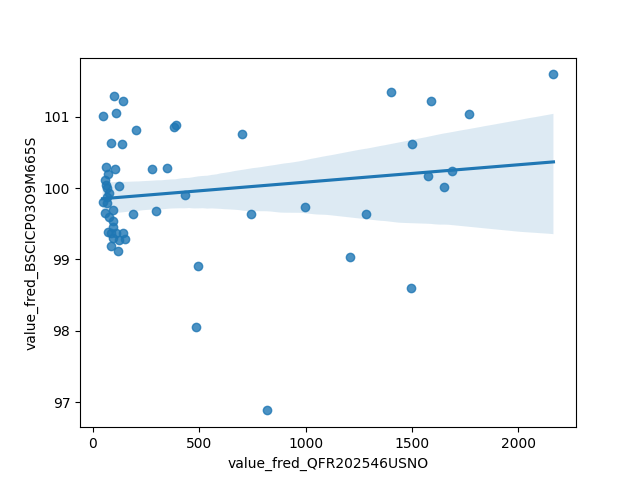
\includegraphics[scale = 0.9]{plots/plot_2024-10-28.png}
\caption{Regression Plot for 2024-10-28}
\end{figure}
\newpage

\section{Date: 2024-10-29}
\noindent \textbf{Series ID: WFRBSN40170} 

\noindent This series is titled Share of Debt Securities Held by the 50th to 90th Wealth Percentiles and has a frequency of Quarterly. The units are Percent of Aggregate and the seasonal adjustment is Not Seasonally Adjusted.The observation start date is 1989-07-01 and the observation end date is 2024-04-01.The popularity of this series is 1. \\ 

\noindent \textbf{Series ID: INVDEF} 

\noindent This series is titled Investment Deflator and has a frequency of Quarterly. The units are Index 2012=100 and the seasonal adjustment is Seasonally Adjusted.The observation start date is 1947-01-01 and the observation end date is 2023-10-01.The popularity of this series is 10. \\ 

\subsection{Regression Tables and Plots}
\begin{center}
\begin{tabular}{lclc}
\toprule
\textbf{Dep. Variable:}           & value\_fred\_INVDEF & \textbf{  R-squared:         } &     0.413   \\
\textbf{Model:}                   &         OLS         & \textbf{  Adj. R-squared:    } &     0.409   \\
\textbf{Method:}                  &    Least Squares    & \textbf{  F-statistic:       } &     95.66   \\
\textbf{Date:}                    &   Tue, 29 Oct 2024  & \textbf{  Prob (F-statistic):} &  1.96e-17   \\
\textbf{Time:}                    &       20:33:20      & \textbf{  Log-Likelihood:    } &   -404.25   \\
\textbf{No. Observations:}        &           138       & \textbf{  AIC:               } &     812.5   \\
\textbf{Df Residuals:}            &           136       & \textbf{  BIC:               } &     818.4   \\
\textbf{Df Model:}                &             1       & \textbf{                     } &             \\
\textbf{Covariance Type:}         &      nonrobust      & \textbf{                     } &             \\
\bottomrule
\end{tabular}
\begin{tabular}{lcccccc}
                                  & \textbf{coef} & \textbf{std err} & \textbf{t} & \textbf{P$> |$t$|$} & \textbf{[0.025} & \textbf{0.975]}  \\
\midrule
\textbf{const}                    &     134.7819  &        2.656     &    50.741  &         0.000        &      129.529    &      140.035     \\
\textbf{value\_fred\_WFRBSN40170} &      -1.5998  &        0.164     &    -9.781  &         0.000        &       -1.923    &       -1.276     \\
\bottomrule
\end{tabular}
\begin{tabular}{lclc}
\textbf{Omnibus:}       & 15.344 & \textbf{  Durbin-Watson:     } &    0.027  \\
\textbf{Prob(Omnibus):} &  0.000 & \textbf{  Jarque-Bera (JB):  } &    6.459  \\
\textbf{Skew:}          &  0.285 & \textbf{  Prob(JB):          } &   0.0396  \\
\textbf{Kurtosis:}      &  2.106 & \textbf{  Cond. No.          } &     111.  \\
\bottomrule
\end{tabular}
%\caption{OLS Regression Results}
\end{center}

Notes: \newline
 [1] Standard Errors assume that the covariance matrix of the errors is correctly specified.

\begin{figure}
\centering
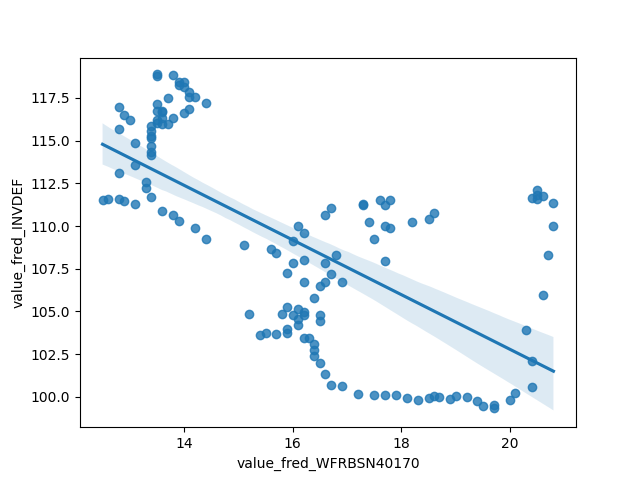
\includegraphics[scale = 0.9]{plots/plot_2024-10-29.png}
\caption{Regression Plot for 2024-10-29}
\end{figure}
\newpage

\section{Date: 2024-10-30}
\noindent \textbf{Series ID: DISC6221ALLEST176QNSA} 

\noindent This series is titled Total Discharges for General Medical and Surgical Hospitals, All Establishments and has a frequency of Quarterly. The units are Thousands of Units and the seasonal adjustment is Not Seasonally Adjusted.The observation start date is 2012-07-01 and the observation end date is 2024-04-01.The popularity of this series is 0. \\ 

\noindent \textbf{Series ID: CES4300000034} 

\noindent This series is titled Indexes of Aggregate Weekly Hours of Production and Nonsupervisory Employees, Transportation and Warehousing and has a frequency of Monthly. The units are Index 2002=100 and the seasonal adjustment is Seasonally Adjusted.The observation start date is 1972-01-01 and the observation end date is 2024-09-01.The popularity of this series is 1. \\ 

\subsection{Regression Tables and Plots}
\begin{center}
\begin{tabular}{lclc}
\toprule
\textbf{Dep. Variable:}                     & value\_fred\_CES4300000034 & \textbf{  R-squared:         } &     0.344   \\
\textbf{Model:}                             &            OLS             & \textbf{  Adj. R-squared:    } &     0.330   \\
\textbf{Method:}                            &       Least Squares        & \textbf{  F-statistic:       } &     24.12   \\
\textbf{Date:}                              &      Wed, 30 Oct 2024      & \textbf{  Prob (F-statistic):} &  1.19e-05   \\
\textbf{Time:}                              &          19:57:57          & \textbf{  Log-Likelihood:    } &   -197.22   \\
\textbf{No. Observations:}                  &               48           & \textbf{  AIC:               } &     398.4   \\
\textbf{Df Residuals:}                      &               46           & \textbf{  BIC:               } &     402.2   \\
\textbf{Df Model:}                          &                1           & \textbf{                     } &             \\
\textbf{Covariance Type:}                   &         nonrobust          & \textbf{                     } &             \\
\bottomrule
\end{tabular}
\begin{tabular}{lcccccc}
                                            & \textbf{coef} & \textbf{std err} & \textbf{t} & \textbf{P$> |$t$|$} & \textbf{[0.025} & \textbf{0.975]}  \\
\midrule
\textbf{const}                              &     380.4686  &       49.588     &     7.673  &         0.000        &      280.653    &      480.284     \\
\textbf{value\_fred\_DISC6221ALLEST176QNSA} &      -0.0273  &        0.006     &    -4.911  &         0.000        &       -0.039    &       -0.016     \\
\bottomrule
\end{tabular}
\begin{tabular}{lclc}
\textbf{Omnibus:}       &  3.469 & \textbf{  Durbin-Watson:     } &    0.481  \\
\textbf{Prob(Omnibus):} &  0.176 & \textbf{  Jarque-Bera (JB):  } &    2.867  \\
\textbf{Skew:}          & -0.598 & \textbf{  Prob(JB):          } &    0.238  \\
\textbf{Kurtosis:}      &  3.041 & \textbf{  Cond. No.          } & 2.04e+05  \\
\bottomrule
\end{tabular}
%\caption{OLS Regression Results}
\end{center}

Notes: \newline
 [1] Standard Errors assume that the covariance matrix of the errors is correctly specified. \newline
 [2] The condition number is large, 2.04e+05. This might indicate that there are \newline
 strong multicollinearity or other numerical problems.

\begin{figure}
\centering
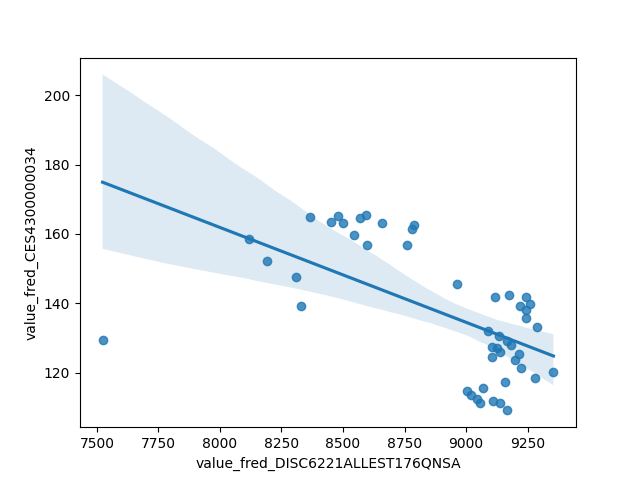
\includegraphics[scale = 0.9]{plots/plot_2024-10-30.png}
\caption{Regression Plot for 2024-10-30}
\end{figure}
\newpage

\section{Date: 2024-10-31}
\noindent \textbf{Series ID: NCOTOT35} 

\noindent This series is titled Total Net Loan Charge-offs to Total Loans, Banks with Total Assets from $1B to $10B, South Atlantic Census Division (DISCONTINUED) and has a frequency of Quarterly, End of Period. The units are Percent and the seasonal adjustment is Not Seasonally Adjusted.The observation start date is 1988-01-01 and the observation end date is 2020-07-01.The popularity of this series is 1. \\ 

\noindent \textbf{Series ID: SWSTFININSREALQGSP} 

\noindent This series is titled Chain-Type Quantity Index for Real GDP: Finance, Insurance, Real Estate, Rental, and Leasing (52, 53) in the Southwest BEA Region and has a frequency of Annual. The units are Index 2017=100 and the seasonal adjustment is Not Seasonally Adjusted.The observation start date is 1997-01-01 and the observation end date is 2023-01-01.The popularity of this series is 1. \\ 

\subsection{Regression Tables and Plots}
\begin{center}
\begin{tabular}{lclc}
\toprule
\textbf{Dep. Variable:}        & value\_fred\_SWSTFININSREALQGSP & \textbf{  R-squared:         } &     0.251   \\
\textbf{Model:}                &               OLS               & \textbf{  Adj. R-squared:    } &     0.217   \\
\textbf{Method:}               &          Least Squares          & \textbf{  F-statistic:       } &     7.360   \\
\textbf{Date:}                 &         Thu, 31 Oct 2024        & \textbf{  Prob (F-statistic):} &   0.0127    \\
\textbf{Time:}                 &             14:26:50            & \textbf{  Log-Likelihood:    } &   -98.241   \\
\textbf{No. Observations:}     &                  24             & \textbf{  AIC:               } &     200.5   \\
\textbf{Df Residuals:}         &                  22             & \textbf{  BIC:               } &     202.8   \\
\textbf{Df Model:}             &                   1             & \textbf{                     } &             \\
\textbf{Covariance Type:}      &            nonrobust            & \textbf{                     } &             \\
\bottomrule
\end{tabular}
\begin{tabular}{lcccccc}
                               & \textbf{coef} & \textbf{std err} & \textbf{t} & \textbf{P$> |$t$|$} & \textbf{[0.025} & \textbf{0.975]}  \\
\midrule
\textbf{const}                 &      93.4795  &        4.655     &    20.084  &         0.000        &       83.827    &      103.132     \\
\textbf{value\_fred\_NCOTOT35} &     -10.9956  &        4.053     &    -2.713  &         0.013        &      -19.401    &       -2.590     \\
\bottomrule
\end{tabular}
\begin{tabular}{lclc}
\textbf{Omnibus:}       &  8.287 & \textbf{  Durbin-Watson:     } &    0.166  \\
\textbf{Prob(Omnibus):} &  0.016 & \textbf{  Jarque-Bera (JB):  } &    2.108  \\
\textbf{Skew:}          &  0.166 & \textbf{  Prob(JB):          } &    0.348  \\
\textbf{Kurtosis:}      &  1.586 & \textbf{  Cond. No.          } &     2.66  \\
\bottomrule
\end{tabular}
%\caption{OLS Regression Results}
\end{center}

Notes: \newline
 [1] Standard Errors assume that the covariance matrix of the errors is correctly specified.

\begin{figure}
\centering
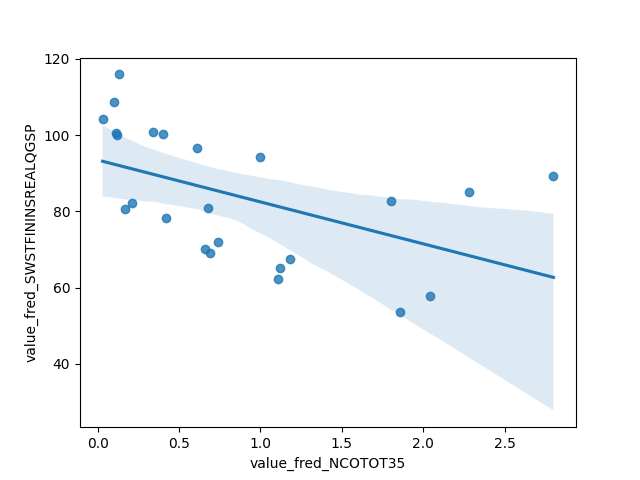
\includegraphics[scale = 0.9]{plots/plot_2024-10-31.png}
\caption{Regression Plot for 2024-10-31}
\end{figure}
\newpage

\section{Date: 2024-11-01}
\noindent \textbf{Series ID: BA6M} 

\noindent This series is titled 6-Month Bankers Acceptance Rate (DISCONTINUED) and has a frequency of Monthly. The units are Percent and the seasonal adjustment is Not Seasonally Adjusted.The observation start date is 1976-01-01 and the observation end date is 2000-06-01.The popularity of this series is 3. \\ 

\noindent \textbf{Series ID: BSBUCT01DEM460S} 

\noindent This series is titled Business Tendency Surveys for Manufacturing: Business Situation: Current: National Indicator for Germany (DISCONTINUED) and has a frequency of Monthly. The units are Net Percent and the seasonal adjustment is Seasonally Adjusted.The observation start date is 1961-01-01 and the observation end date is 2013-09-01.The popularity of this series is 1. \\ 

\subsection{Regression Tables and Plots}
\begin{center}
\begin{tabular}{lclc}
\toprule
\textbf{Dep. Variable:}    & value\_fred\_BSBUCT01DEM460S & \textbf{  R-squared:         } &     0.027   \\
\textbf{Model:}            &             OLS              & \textbf{  Adj. R-squared:    } &     0.024   \\
\textbf{Method:}           &        Least Squares         & \textbf{  F-statistic:       } &     8.216   \\
\textbf{Date:}             &       Fri, 01 Nov 2024       & \textbf{  Prob (F-statistic):} &  0.00445    \\
\textbf{Time:}             &           14:42:21           & \textbf{  Log-Likelihood:    } &   -1224.5   \\
\textbf{No. Observations:} &               294            & \textbf{  AIC:               } &     2453.   \\
\textbf{Df Residuals:}     &               292            & \textbf{  BIC:               } &     2460.   \\
\textbf{Df Model:}         &                 1            & \textbf{                     } &             \\
\textbf{Covariance Type:}  &          nonrobust           & \textbf{                     } &             \\
\bottomrule
\end{tabular}
\begin{tabular}{lcccccc}
                           & \textbf{coef} & \textbf{std err} & \textbf{t} & \textbf{P$> |$t$|$} & \textbf{[0.025} & \textbf{0.975]}  \\
\midrule
\textbf{const}             &       3.4192  &        2.455     &     1.393  &         0.165        &       -1.412    &        8.250     \\
\textbf{value\_fred\_BA6M} &      -0.8848  &        0.309     &    -2.866  &         0.004        &       -1.492    &       -0.277     \\
\bottomrule
\end{tabular}
\begin{tabular}{lclc}
\textbf{Omnibus:}       & 11.375 & \textbf{  Durbin-Watson:     } &    0.040  \\
\textbf{Prob(Omnibus):} &  0.003 & \textbf{  Jarque-Bera (JB):  } &   10.376  \\
\textbf{Skew:}          & -0.398 & \textbf{  Prob(JB):          } &  0.00558  \\
\textbf{Kurtosis:}      &  2.539 & \textbf{  Cond. No.          } &     21.7  \\
\bottomrule
\end{tabular}
%\caption{OLS Regression Results}
\end{center}

Notes: \newline
 [1] Standard Errors assume that the covariance matrix of the errors is correctly specified.

\begin{figure}
\centering
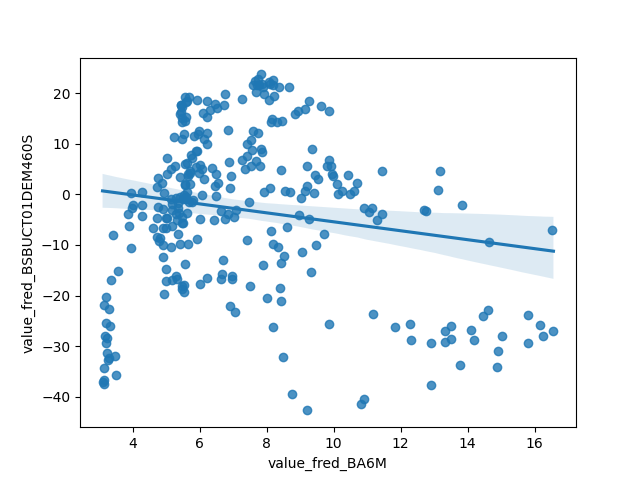
\includegraphics[scale = 0.9]{plots/plot_2024-11-01.png}
\caption{Regression Plot for 2024-11-01}
\end{figure}
\newpage

\include{tex_things/day_2024-11-02}
\include{tex_things/day_2024-11-03}

\end{document}
